\section{Overview}
\label{sec:overview}

% You may need to move this \begin{figure} ... \end{figure} block around
% in the document to place it in a logical spot in the paper. In
% general, get the figure on the same page as the prose that refers to
% it.
\begin{figure}[t]
  \centering
  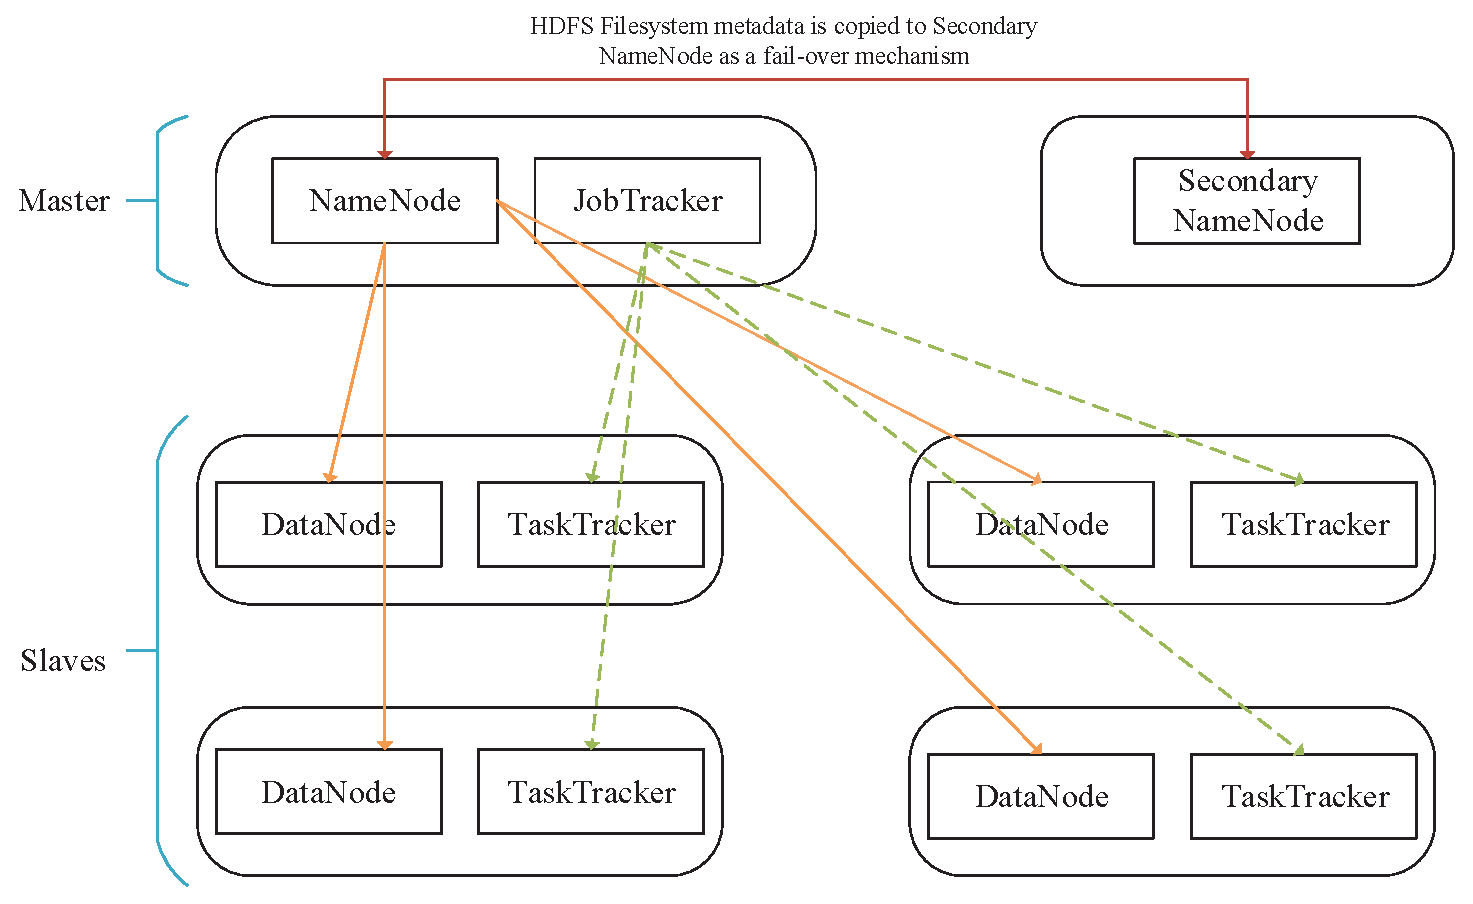
\includegraphics[width=3in]{figs/HadoopOverview.eps}
  \caption{Hadoop 1.x Architecture Overview}
  \label{fig:hadoop1.xoverview}
\end{figure}
In this section, we first talk about the architecture and components in Hadoop 1.x and Hadoop 2.x. We point out issues unsolved in Hadoop 2.x. Then we introduce Docker, compare Docker with other container technologies, and discuss the impact of incorporating the Docker container into Hadoop.
\subsection{Hadoop}

Hadoop is an open-source software for large-scale data processing with commodity machines. It could scale up from a single server to thousands of machines, with very high degree of fault tolerance. Since Hadoop assumes each machine is prone to failures, the resiliency of Hadoop clusters comes from the software's ability to detect and handle failures at the application layer instead of relying on high-end hardware, 

Hadoop Distributed File System(HDFS) and MapReduce~\cite{dean2008mapreduce} are the two core components of Hadoop. HDFS is a distributed file system that provides high-through access to application data while MapReduce is a framework for parallel processing of large data sets. Figure \ref{fig:hadoop1.xoverview} presents the architecture for Hadoop 1.x. The main components of HDFS are the NameNode, the DataNodes, and the SecondaryNameNode. The NameNode is the master of the system which maintains the name system (directories and files) and manages the blocks which are stored on the DataNodes. The DataNodes are the slaves which are deployed on each machine and provide the actual storage. The SecondaryNameNode is {\em not} a back up server of the Namenode, but instead is responsible for performing periodic checkpoints for the HDFS system file(i.e.,fsimage). The main components of MapReduce are the JobTracker and the Tasktrackers. The JobTracker is the master of the system which manages the jobs and resources in the cluster. The TaskTrackers are the slaves which are deployed on each machine. They are responsible for running the Map and Reduce tasks under the instruction from the JobTracker.

%\iffalse
%The most important aspect of Hadoop is that both HDFS and MapReduce are designed with each other in mind and each are co-deployed such that there is a single cluster and thus provides the ability to move computation to the data not the other way around. Thus, the storage system is not physically separate from a processing system.
%\fi

However, Hadoop 1.x is not scalable enough and has many limitations. Firstly, there is no horizontal scalability of the NameNode and it does not support the NameNode High Availability. Specifically, it can only support up to 4,000 nodes per cluster and there is always only one NameNode server. Secondly, the JobTracker becomes the bottleneck of Hadoop because it is responsible for both resource management and job scheduling and is easily to become overburdened. Finally, the storage system (i.e., HDFS) is not physically separated from the data processing system (i.e., MapReduce). Both HDFS and MapReduce are designed with each other in mind and each are co-deployed. It takes advantages of data locality and provides the ability to move computation to the data not the other way around.

\begin{figure}[t]
  \centering
  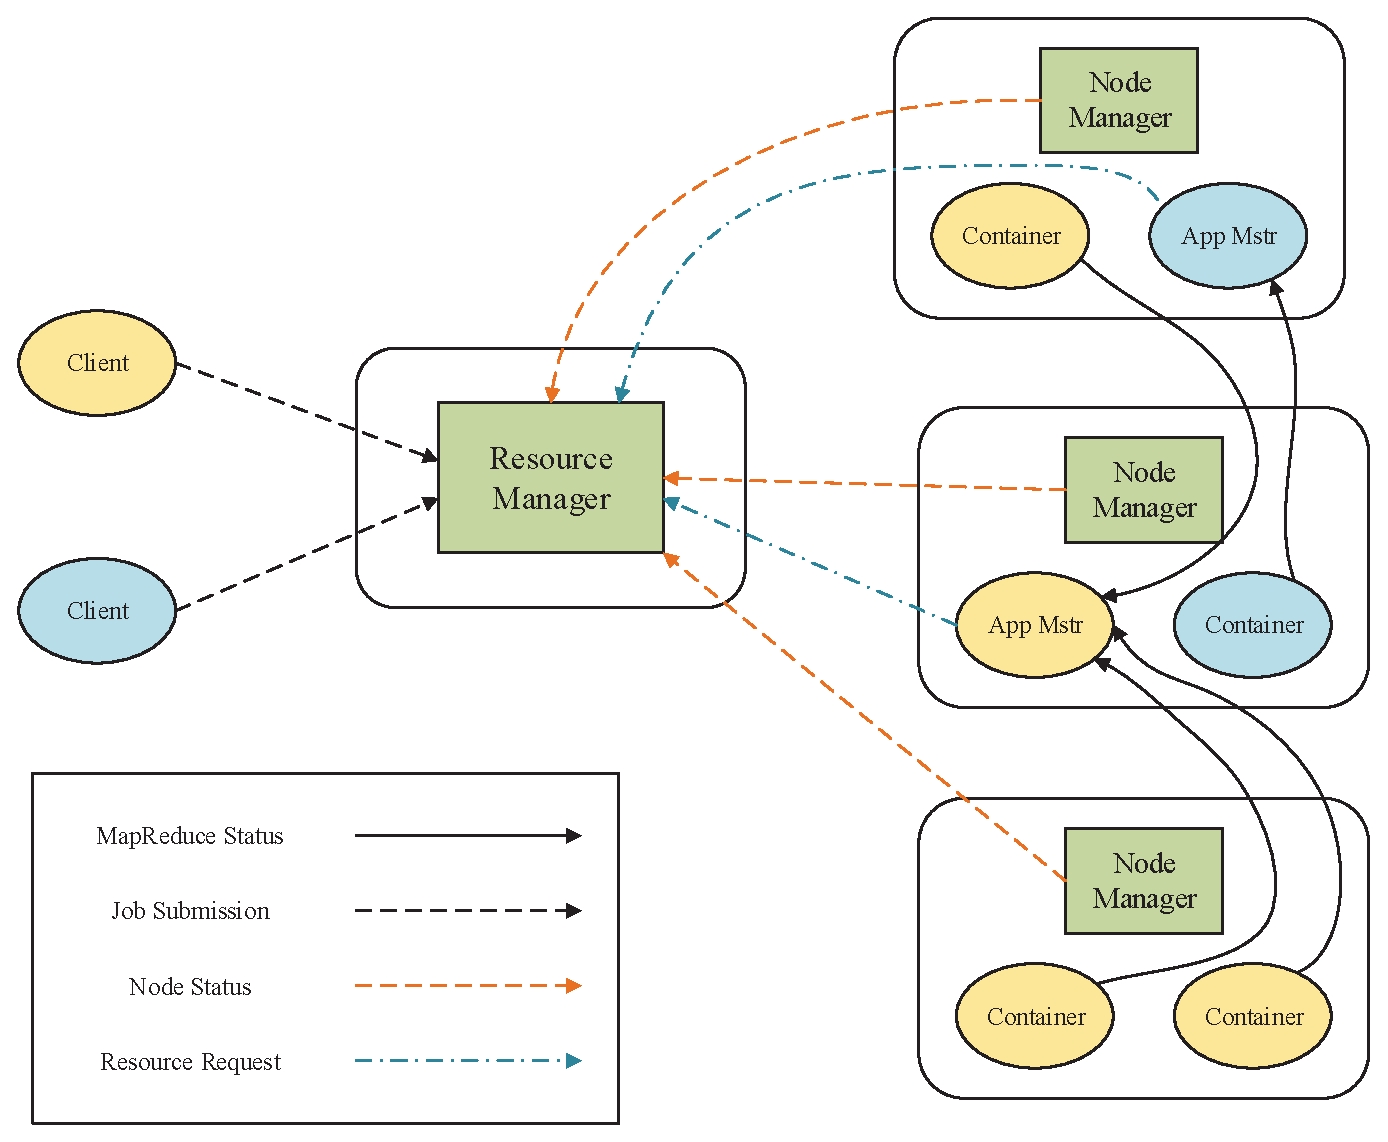
\includegraphics[width=3in]{figs/yarn.eps}
  \caption{Hadoop YARN components}
  \label{fig:yarnoverview}
\end{figure}

Hadoop 2.x is developed to handle the scalability problem in Hadoop with a new component called Hadoop YARN (Yet Another Resource Negotiator)~\cite{vavilapalli2013apache}. Haoop 2.x splits up the two major functionalities of the JobTracker, resource management and job scheduling, into separate daemons. HDFS does not change in Hadoop 2.x. The YARN component is introduced to replace JobTracker. As shown in Figure \ref{fig:yarnoverview}, YARN has three types of components: the ResourceManager, the NodeManager, and the ApplicationMaster. The ResourceManager is the master that arbitrates all the available cluster resources and thus helps manage the distributed applications running on the YARN system. The NodeManager is YARN’s per-node agent, and takes care of the individual compute nodes in a Hadoop cluster, such as keeping up-to date with the ResourceManager, overseeing containers’ life-cycle management, monitoring resource usage (memory, CPU) of individual containers, etc. The ApplicationMaster is, in effect, an instance of a framework-specific library and is responsible for negotiating resources from the ResourceManager and working with the NodeManagers to execute and monitor the containers and their resource consumption. It has the responsibility of negotiating appropriate resource containers from the ResourceManager, tracking their status and monitoring progress. As discussed above, Hadoop 2.x only solves the second problem of Hadoop 1.x. The problems related to HDFS are not solved yet.

\subsection{Docker in Hadoop}
Docker is an open platform for developing, shipping, and running applications. It is a Linux-based system that automates the deployment of applications inside software containers, by providing an additional layer of abstraction and automation of operating system level virtualization on Linux. Docker uses resource isolation features of the Linux kernel such as cgroups, and kernel namespace to allow independent "containers" to run within a single Linux instance, avoiding the overhead of starting virtual machines. With Docker we can separate our applications form the infrastructure and treat the infrastructure like a managed application. 

As we can see from the Figure \ref{fig:Dockeroverview}, the Docker Engine Container compromises just the application and its dependencies. It provides a way to run almost any application securely isolated in a container. It runs as an isolated process in user space on the host operating system, sharing the kernel with other containers, so that many containers are allowed to run simultaneously on the host. 
\begin{figure}[t]
  \centering
  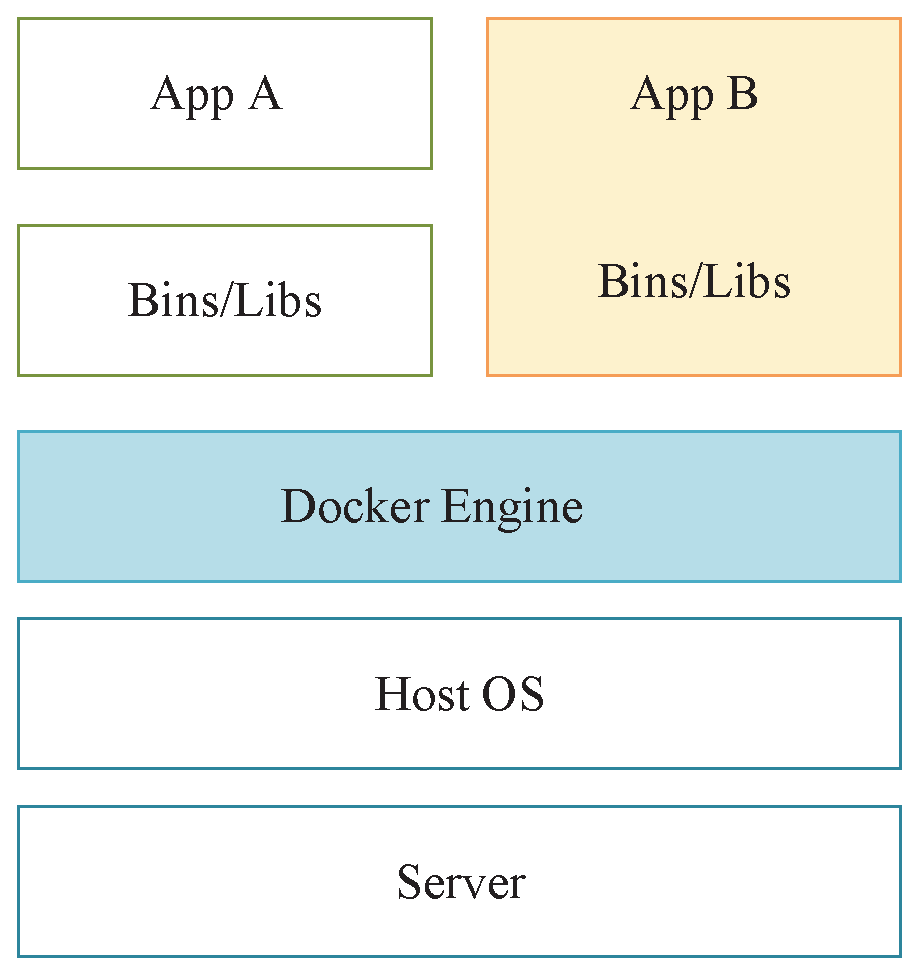
\includegraphics[width=2in]{figs/docker.eps}
  \caption{Docker}
  \label{fig:Dockeroverview}
\end{figure}

Compared to Virtual Machines(VMs), Docker container provides more resource sharing, less isolation, and weaker security. Each VM has its own different OS and  is portable to all type of OSes(e.g., Linux, Windows, OS X). But all Docker containers share the same host OS kernel and limited to Linux at the moment. While VMs are isolated through emulation and only hardware are shared, Docker containers are only isolated by system kernel virtualization. That means Docker containers only have different views of the operating system and some kernel subsystems and devices are shared across containers (e.g., SELinux, Cgroups, /sys, /proc/sys). The lightweight nature of containers means it enjoys the resource isolation and allocation benefits of virtual machines but is much more efficient, and suffers the security vulnerabilities brought by the resource sharing.

Docker used to use Linux Continaers(LXC)~\cite{helsley2009lxc} to provide isolated Linux virtual environment for containers, but has dropped LXC and replaced LXC with its own libraries~\cite{droplxc} for isolated environment. Both LXC and Docker are container technologies. Their difference is that LXC provides base OS containers while Docker provides single application virtualization based on containers. LXC containers can be treated as an OS and applications and services can be installed inside the container. However, Docker containers are limited to a single application and could not install other applications. This is because the Docker container is restricted to just one single process and could not support multiple applications with multiple processes. In summary, Docker is not just an alternative for LXC and offers high-level services for application containers(e.g., layered file system isolation, image management).

OpenVZ~\cite{openvz} and FreeBSD Jails~\cite{jails} also belong to containerization systems. FreeBSD Jails is a non-Linux containerization system and an enhancement to chroot. Besides resource isolation, FreeBSD Jails provides segregation of users, processes, and networks as well. Similar to LXC, OpenVZ is a Linux container solution. While OpenVZ, FreeBSD Jails, and Docker all provide application virtualizaiton, Docker also provides application portability through the Docker container images.

Docker has recently been officially integrated into Hadoop 2.0(YARN), where big data tasks such as MapReduce mappers and reducers run on individual containers. The marriage of Hadoop jobs with containers offers considerable benefits compared to running these jobs on VMs(in Hadoop 1.0). These include shorter provisioning time, more light weight migration, better performance isolation, bypassing virtual I/Os, and higher resource utilization since a single machine can accommodate more containers than VMs. 

Hadoop YARN container represents a collection of physical resources, including CPU cores, disk along with RAM. Docker container can perfectly implement this concept. By using Docker containers, resources can be isolated, services restricted, and processes provisioned to have a private view of the operating system with their own process ID space, file system structure, and network interfaces. Docker Container Executor (DCE) is thus developed. Other container executors are Default Container Executor and Linux Container Executor which is implemented with cgroups.

